\documentclass[conference]{IEEEtran}
% \IEEEoverridecommandlockouts
% The preceding line is only needed to identify funding in the first footnote. If that is unneeded, please comment it out.
\usepackage{cite}
\usepackage{amsmath,amssymb,amsfonts}
\usepackage{algorithmic}
\usepackage{graphicx}
\usepackage{textcomp}
\usepackage{xcolor}
\usepackage{hyperref}
\usepackage{xurl}
\newcommand{\repourl}{\url{https://github.com/bmp/pota-india-hfi2026}}
\def\BibTeX{{\rm B\kern-.05em{\sc i\kern-.025em b}\kern-.08em
    T\kern-.1667em\lower.7ex\hbox{E}\kern-.125emX}}

\begin{document}
\title{Parks on the Air (POTA) in India: Current Operational Status and Pathways for Participation}

% TODO: add affiliation and city if required
\author{\IEEEauthorblockN{Bharath M. Palavalli (VU3GLJ)}
\IEEEauthorblockA{vu3glj@disroot.org\\
\url{https://ham.bharathpalavalli.com}}}

\maketitle
\IEEEpubid{\makebox[\columnwidth]{\hfill \begin{minipage}{\textwidth}
\centering
\vspace{7\baselineskip} % increase this to push it lower
HAMFEST INDIA-2026, NITK Surathkal \copyright
\end{minipage}
}}
\IEEEpubidadjcol

\begin{abstract}
This exploratory paper presents a preliminary, data-driven analysis of
Parks on the Air (POTA) operations within India. While portable
amateur radio operations have seen a global surge, participation
within this region remains comparatively low. The spatial and temporal
distribution across 191 listed parks reveals significant inequality,
with 141 parks remaining unactivated. Through a combination of
international contest logs, digital logbooks, and automated spotting
networks (RBN, PSKReporter, WSPRnet), the author established an
initial set of 481 digitally verifiable, active high-frequency (HF)
licensed amateur radio operators active since 2024 in India. However,
only 19 such operators have participated in POTA activations since
2021. This paper then provides hypotheses for this low activity,
including regulatory hurdles and equipment accessibility. The paper
outlines actionable community strategies to foster growth in POTA
operations in India.
\end{abstract}

\begin{IEEEkeywords}
Amateur Radio, Parks on the Air, Portable Operations, Exploratory Data
Analysis, HF Operations, Field Operations
\end{IEEEkeywords}

\section{Introduction}
Amateur radio has a tradition of field operations, ranging from
informal outings to official International Amateur Radio Union (IARU)
field days. This ecosystem includes contests organized by national
societies and local clubs, alongside events focused on specific bands,
modes, or equipment constraints (e.g., low-power, home-brewed). These
initiatives aim to popularize the hobby, test equipment, and bolster
emergency preparedness. In India, the Amateur Radio Society of India
(ARSI)\footnote{From \url{https://arsi.info/}: ARSI is the
  IARU-recognized national association for amateur radio operators in
  India. (Last accessed: 10 Jul 2026).} organizes events such as the
National Field Day \& Hill Topping Contest, the ARSI QRP-DAY Contest,
and the ARSI VU-DX Contest (many local clubs and societies in India
organize their own versions of these field operations).

While many activities are date-specific, the following programs
operate continuously:
\begin{itemize}
    \item \textbf{Parks on the Air (POTA):} Encourages portable
      deployments from designated parks \cite{b7}, requiring 10 QSOs
      on a single UTC day for a successful
      activation\footnote{\url{https://docs.pota.app/docs/rules.html\#activations--attempts}
        (Last accessed: 10 Jul 2026).}.
    \item \textbf{World Wide Flora \& Fauna (WWFF):} Promotes
      operations from protected nature reserves \cite{b8}, requiring
      44 QSOs for a successful
      activation\footnote{\url{https://wwff.co/rules-faq/how-to-activate-a-wwff-reference/}
        (Last accessed: 10 Jul 2026).}.
    \item \textbf{Summits on the Air (SOTA):} An award scheme for
      activating mountain summits \cite{b9}.
\end{itemize}

This paper focuses on POTA activity. Unlike the robust participation
seen in U.S. POTA analyses \cite{b1}, the Indian footprint remains
limited. Inspired by this analysis, this study investigates the
distribution, and growth of POTA activities in India. By analyzing
current operations, this paper hypothesizes barriers to entry, and
proposes approaches for community-driven improvement.

\section{Approach}
\label{sec:methodology}
To understand POTA in India, this section outlines the approach for
identifying both available national parks and the active HF operator
base.

\subsection{List of Active Parks}
While India has a network of 1014 Protected Areas including 106
National Parks, 573 Wildlife Sanctuaries, 115 Conservation Reserves
and 220 Community Reserves~\cite{b10}, not all of these parks are
listed on the POTA site. In order to establish the baseline of
available entities, geo-spatial and activation data for Indian parks
were obtained using Python scripts, which fetched the data from the
official Parks on the Air (POTA) API
(\url{https://api.pota.app/program/parks/IN}). This endpoint provided
the complete list of 191 designated POTA entities in the country,
including their geographical coordinates and current activation
status, which were subsequently mapped against the GeoJSON vector
outline of India.

\subsection{Active Licensed Amateur Radio Operators}
Ascertaining the true number of active HF amateur radio operators in
India poses a challenge due to the lack of publicly available,
centralized regulatory data. While the HAMFEST 2026 registration lists
590 registered licensed HAMs~\cite{b2} as participants, verifiable
on-air activity is a challenging task.

This study employs a dual-methodology census relying entirely on open
data endpoints:
\begin{enumerate}
    \item \textit{Intentional Log Uploaders (Three-Year Baseline):}
      Operators actively uploading logs to the Logbook of The World
      (LoTW) \cite{b4}, the POTA database \cite{b3}, and public
      contest submissions (including CQ WPX, CQ WW, and ARRL contests)
      \cite{b5} between 2024 and 2026.
    \item \textit{Active RF Emitters (Recent Snapshots):} To account
      for operators who transmit but do not participate in logging
      platforms or contests, data was aggregated from automated
      spotting networks, including the Reverse Beacon Network (RBN)
      \cite{b6} and PSKReporter \cite{b11} over the most recent
      24-hour period, and WSPRnet \cite{b12} using its most recent
      monthly archive.
    \end{enumerate}

Two limitations of this approach must be noted: 1) proprietary logging
platforms such as QRZ.com--which is widely used by licensed radio
operators in India to upload logs and establish their
activity--restrict automated data access through premium APIs and
anti-bot protections, preventing their inclusion; and 2) the data
collection focuses exclusively on digitally verifiable HF footprints,
thereby omitting purely local operators who rely entirely on VHF/UHF
repeaters or traditional operators who solely maintain paper logs.
While these omissions may under-represent the absolute total count of
active operators in the country, this trade-off is acceptable for the scope
of this study. The analysis is specifically interested in HF operators
who are actively interacting with the global community, uploading
their logs to online platforms, and potentially using programs such as
POTA.

\section{Results and Analysis}

\subsection{Park Distribution and Activation Status}
As seen in Fig.~\ref{fig:map}, there are currently 191 designated POTA
entities in India. Of these, 50 parks have been activated a total of
104 times. In comparison, there are almost 12,000 parks listed on POTA for
the United States of America, most of which have been activated at
least once~\cite{b1}. The geographical spread indicates that states
such as West Bengal, Karnataka, and Madhya Pradesh, account for the
majority of the activation volume.

\begin{figure}[htbp]
\centerline{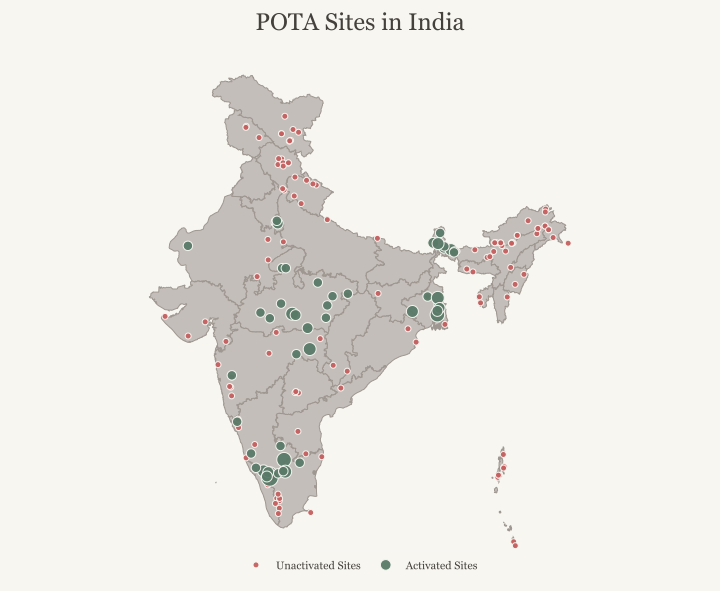
\includegraphics[width=\linewidth]{POTA_India_Map.png}}
\caption{Geographical distribution of unactivated and activated POTA
  sites across India.}
\label{fig:map}
\end{figure}

A significant disparity exists within the activation data. Currently,
141 listed parks (73.8\%) remain unactivated. As seen in Table~\ref{tab:activation-tiers}, 30 parks have been activated only once,
while far fewer parks have been activated more than once.
Sixteen parks have been activated between 2 to 5 times, and four parks
have been activated between 6 to 10 times. No park has been activated
more than ten times until the time of preparing this manuscript.

\begin{table}[htbp]
\caption{Breakdown of POTA Parks by Activation Tiers}
\begin{center}
\begin{tabular}{lc}
\hline
\textbf{Activation Tier} & \textbf{Number of Parks} \\
\hline
Unactivated & 141 \\
1 Activation & 30 \\
2 to 5 Activations & 16 \\
6 to 10 Activations & 4 \\
11+ Activations & 0 \\
\hline
\end{tabular}
\label{tab:activation-tiers}
\end{center}
\end{table}

Furthermore, an analysis of lifetime activations by park rank
demonstrates severe inequality. Notably, just 2 parks (Mudumalai and
Bandipur) account for 18 activations, and the top 4 parks together
have 30 of the 104 activations, which is 28.8\% of all national
activity.

\subsection{Temporal Trends in Activations}

A longitudinal analysis of cumulative completed activations from 2021
to 2026 illustrates a slow rate of adoption (as seen in Fig.~\ref{fig:timeline}). While cumulative totals reached 123 by mid-2026,
the year-over-year rate displayed a minor contraction between 2024 (30
activations) and 2025 (25 activations). However, early data indicates
that 2026 is on pace to register the highest annual activation count
to date.

\begin{figure}[htbp]
\centerline{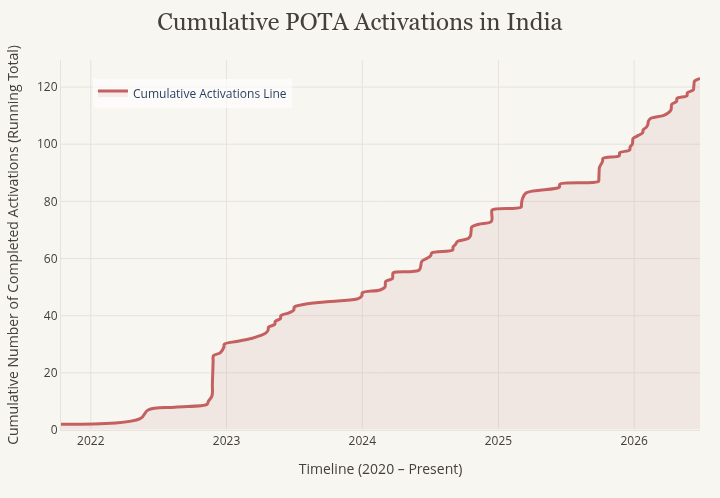
\includegraphics[width=0.75\linewidth]{timeline.png}}
\caption{Cumulative growth of POTA activations in India.}
\label{fig:timeline}
\end{figure}

\subsection{Operator Demographics and Effort}
Based on the approach detailed in Section~\ref{sec:methodology}, the
data list of HF operators was compiled. The inclusion criteria require
operators to be actively interacting with the global community on HF,
participating in global contests, or engaging on platforms such as
POTA. The results of this approach are seen in Table~\ref{tab:active-census-report}. It is interesting to note that the
total discovered operators for POTA alone are 49, whereas when we put
together the list of operators (non-unique) across competitions, the
number is much greater. 247 operators have submitted logs for CQ
competitions, 70 operators submitted logs for IARU contests, and 69
operators submitted logs for ARRL contests.

\begin{table}[htp]
\caption{Unified Active VU HF Operators}
\begin{center}
\resizebox{\columnwidth}{!}{%
\begin{tabular}{lcc}
\hline \textbf{Data Source / Metric} & \textbf{Total Discovered} & \textbf{Extracted Unique} \\ \hline
Logbook of The World (LoTW) & 323 & +323 \\
Parks on the Air (POTA) & 49 & +25 \\
CQ Contests$^a$ & 247 & +53 \\
IARU HF Champ & 70 & +21 \\
ARRL Contests$^b$ & 69 & +6 \\
Reverse Beacon Network (24h) & 69 & +48 \\
PSKReporter (24h) & 12 & +4 \\
WSPRnet (Recent Archive) & 5 & +1 \\
\hline \textbf{Total De-duplicated Active VU} & \textbf{-} & \textbf{481} \\ \hline
\end{tabular}%
}

\vspace{1ex}
\raggedright
\footnotesize
$^a$CQ Contests combined: WPX SSB, WPX CW, WW SSB, WW CW, WW RTTY, WPX
RTTY, 160 CW, and 160 SSB.\\
$^b$ARRL Contests combined: DX CW, DX SSB, RTTY Roundup, 160M,
Sweepstakes CW, Sweepstakes SSB, Int. Digital, and 10M.
\label{tab:active-census-report}
\end{center}
\end{table}

Out of the 481 identified unique active HF operators, only 19
individuals have attempted a park activation, and 17 of them have at
least one successful activation. The community
delivered 123 total activations (104 of which were successful) across
50 unique parks. However, operator effort is highly skewed; as seen
in Fig.~\ref{fig:butterfly} a single operator accounts for 33\% of
all field deployments and nearly 40\% of the dataset's successful
activations.

\begin{figure}[htbp]
\centerline{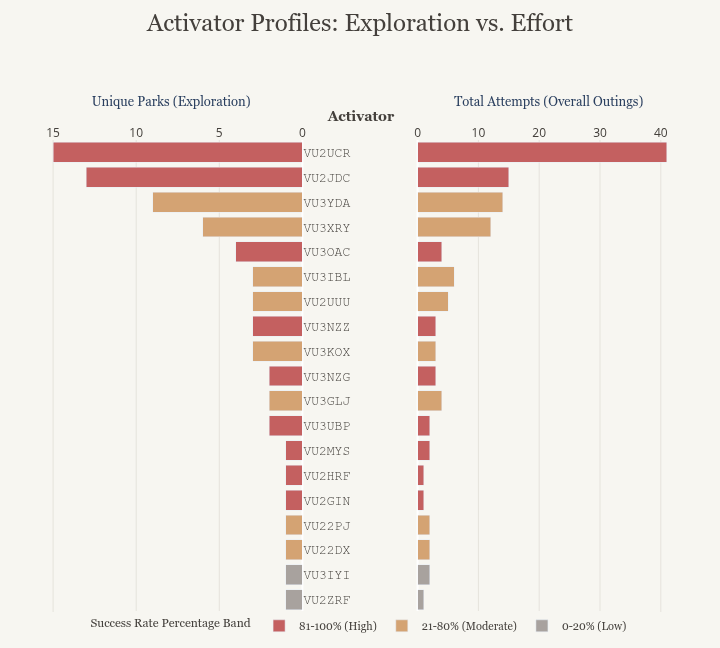
\includegraphics[width=\linewidth]{activator_butterfly.png}}
\caption{Exploration (unique parks) against total activation
  effort of operators}
\label{fig:butterfly}
\end{figure}

The permissible operation criteria (in terms of bands, modes and power
output) for different license classes makes it interesting to analyze
across this parameter. While Indian license classes have undergone
numerous regulatory changes, for the purposes of this study, operators
are categorized heuristically: a VU2 prefix denotes a General Grade
operator, whereas a VU3 prefix denotes a Restricted Grade operator.
When analyzing performance across license classes, unexpected figures
emerge. The sample size of active POTA operators consists of 9 General
Grade and 10 Restricted Grade license holders.

\begin{figure}[htbp]
\centerline{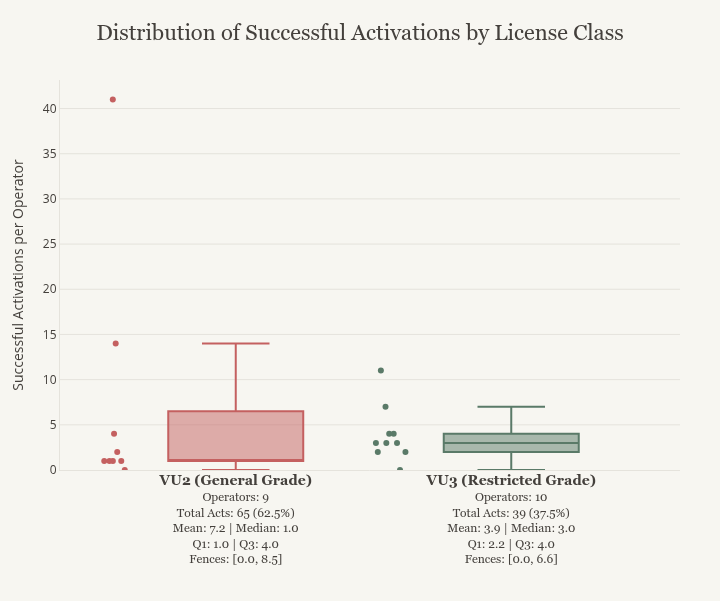
\includegraphics[width=0.75\linewidth]{boxplot.png}}
\caption{Comparison of General and Restricted grade license holders.}
\label{fig:boxplot}
\end{figure}

When correcting for the single high-volume outlier in the General
Grade category, Restricted Grade operators demonstrate a stronger
median (3.0 successful activations versus 1.0) and a higher mean
success rate (3.9 versus 3.0) as seen in Table~\ref{tab:outlier-comparison}. This either indicates that Restricted
Grade operators represent a highly consistent foundation for portable
activity or a greater propensity for HAMs possessing a Restricted
Grade license.

\begin{table}[htbp]
\caption{Impact of Outlier Removal on License Class Statistics}
\begin{center}
\resizebox{\columnwidth}{!}{%
\begin{tabular}{lccc}
\hline \textbf{Metric} & \textbf{General (All)} & \textbf{General (w/o Outlier)} & \textbf{Restricted} \\ \hline
Active Operators & 9 & 8 & 10 \\
Total Attempts & 70 & 29 & 53 \\
Successful ($\geq$10 QSOs) & 65 & 24 & 39 \\
Mean Successful & 7.2 & 3.0 & 3.9 \\
Median Successful & 1.0 & 1.0 & 3.0 \\
\hline
\end{tabular}%
}
\label{tab:outlier-comparison}
\end{center}
\end{table}

\subsection{Geographic Footprint and Exploration}
Understanding operator travel distances provides necessary insight
into deployment logistics. While comprehensive location data exists
behind paywalls on proprietary platforms (e.g., QRZ.com), this study
relies on open-source geographic data from HamQTH to comply with
automated access terms. The polar bearing chart tracks the physical
exploration footprints of activators as seen in Fig.~\ref{fig:polar}.
Radially bound straight lines map out localized activations, while
multi-point runs expand dynamically into continuous filled boundaries
encapsulating the total operational theater. Most operators conduct
activations within a short distance from their primary QTH, with
limited regional travel specifically dedicated to amateur radio
deployments.

\begin{figure}[htbp]
\centerline{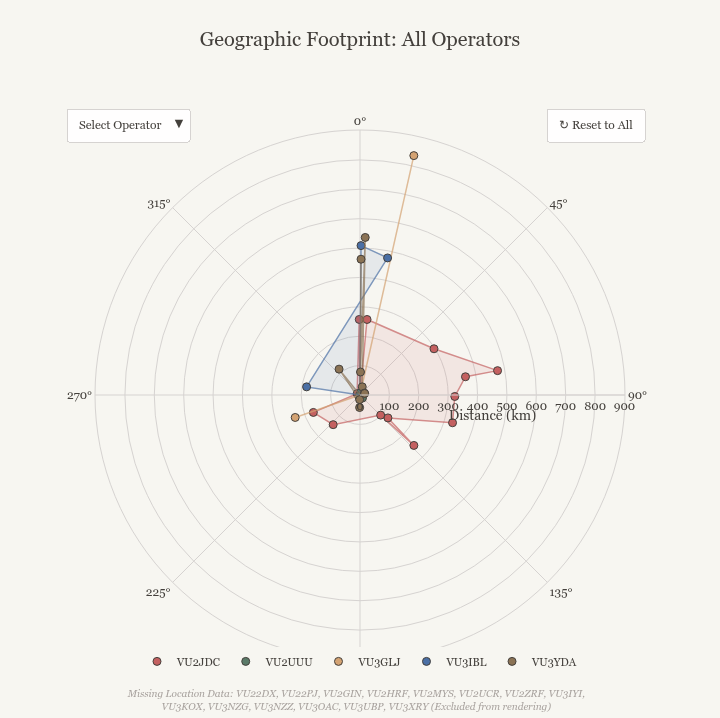
\includegraphics[width=0.75\linewidth]{polar.png}}
\caption{Travel distance of operators$^c$}
\vspace{1ex}
\raggedright
\footnotesize
$^c$Note: This map only has the five activators who have publicly
declared their QTH.
\label{fig:polar}
\end{figure}

While this data is limited to 5 of the 19 operators who activate
parks, the author suspects this is true for most activators apart from
the outlier\footnote{The author has reached out to the other
  activators to confirm that their operations are limited to the parks
  around their geography.}.

\subsection{Hunter Dynamics}
The receiving end of these activations, known as ``Hunters,'' consists
of at least 142 globally distributed operators\footnote{Hunters are
  counted from the POTA park leaderboards, which list at most five
  hunters per park, so this is a lower bound.}. The data indicates that 71\% of
hunters successfully receiving signals from Indian parks are
international (DX) stations, reflecting the strong global demand for
Indian contacts. As seen in Fig.~\ref{fig:hunter} the domestic
hunting landscape is primarily dominated by a small subset of highly
active local operators. Two operators account for 10 and 5 unique
parks, and 26 and 12 confirmed QSOs, respectively.

\begin{figure}[htbp]
\centerline{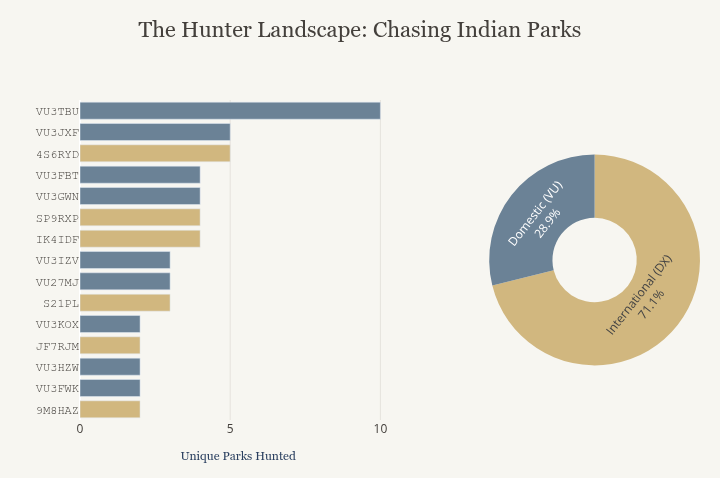
\includegraphics[width=\linewidth]{hunter.png}}
\caption{Distribution and categorization of domestic versus
  international hunters pursuing Indian POTA activations.}
\label{fig:hunter}
\end{figure}

The QSO map of the ``top'' hunters (Fig.~\ref{fig:hunter_map}) can be
interpreted as a result of restricted field operations and band conditions
during operations. There are no hunters from North America, South
America and Africa, this typically matches the band conditions that VU
operators face regularly when using compromised antenna systems, or
operating QRP, or in restricted field conditions.

\begin{figure}[htbp]
\centerline{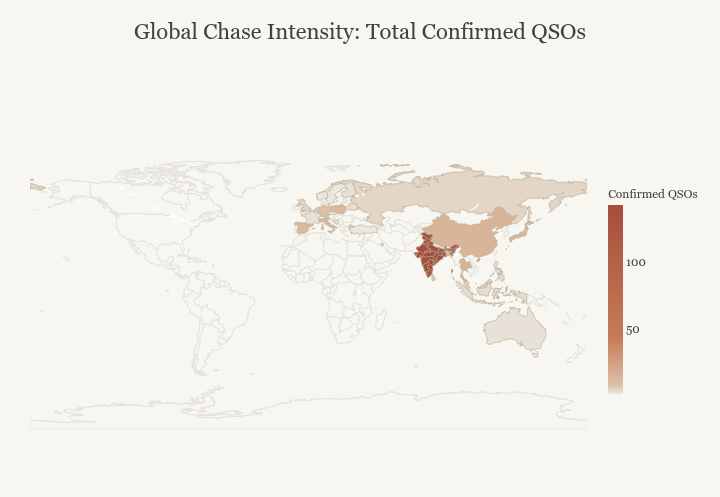
\includegraphics[width=\linewidth]{hunter_map.png}}
\caption{Global choropleth heatmap illustrating the geographic
  distribution of international and domestic operators hunting Indian
  POTA activations.}
\label{fig:hunter_map}
\end{figure}

\subsection{Hypotheses for Low Activity}
\label{subsection:hypotheses}
The data highlights a stark contrast: out of 481 active HF operators,
only 19 have engaged in POTA activities. Several hypotheses emerge for
this low conversion rate:
\begin{enumerate}
    \item \textbf{Regulatory Friction (Park Operations):} Operating
      amateur radio equipment within protected national parks and
      wildlife sanctuaries in India often requires complex
      bureaucratic permissions from local forest departments,
      deterring casual, spontaneous deployments.
    \item \textbf{Regulatory Friction (Transit and Travel):}
      Transporting amateur radio equipment—particularly HF
      transceivers, extensive wire antennas, and high-capacity lithium
      batteries—on domestic flights frequently encounters significant
      security scrutiny and bureaucratic friction, complicating travel
      to remote POTA entities. This occurs despite official
      memorandums and FAQs from the Coordination Wing of the Dept. of
      Telecommunications explicitly clarifying that carrying such
      equipment in India is not restricted \cite{b14, b15}.
    \item \textbf{Equipment Accessibility:} The prohibitive import
      costs and limited domestic availability of lightweight,
      battery-powered HF transceivers (irrespective of QRP rigs or
      otherwise) elevate the financial barrier to entry for portable
      operations.
    \item \textbf{Cultural Operational Preferences:} The current
      domestic amateur radio culture heavily favors fixed-station
      DXing and localized VHF/UHF repeater communications over HF
      field deployments.
    \item \textbf{Aging Operator Demographic:} The active amateur
      radio population skews towards an older demographic that may not
      necessarily seek out the physical demands of remote field
      deployments\footnote{As an anecdote, an exchange within the community after
      the author gave a talk at one of India's oldest radio clubs aptly
      illustrates this skew: when a veteran operator remarked, ``Very
      nice, I often struggle connecting with young people. We need
      young people like you to further our hobby :-)'', and the newly
      licensed operator responded, ``Thank you! HAM is probably the only
      hobby where 40s is considered young :-)''.}.
    \item \textbf{Lack of Post-Event Youth Mentorship:} While annual
      events such as Jamboree on the Air - Jamboree on the Internet
      (JOTA-JOTI)\cite{b13} successfully introduce scouting youth to
      the hobby, there is a distinct lack of structured follow-up
      programs or mentorship pipelines to transition these young
      participants into licensed, active operators who might undertake
      portable operations\footnote{While there are numerous club activities in West
      Bengal and Karnataka that actively reach out to schools and
      colleges for \textit{seminars}, the focus on amateur radio being
      useful only for ``emergency communications'' and the lack of
      experimentation as an entry point tends to discourage entry of
      younger members.}.
    \item \textbf{Park Accessibility:} While India has a network
      of 1,014 Protected Areas, the current list of 191 POTA
      entities is heavily skewed toward remote, highly protected biospheres
      rather than accessible urban or suburban ecological parks,
      requiring significant travel logistics for operators. While this
      could be a result of seeding/pre-seeding that the POTA country
      administrators or the POTA team carried out, it is also
      important to add more ``accessible'' parks that HAMs can access
      easily, and engage with the regulatory authorities to open these
      spaces for POTA activities\footnote{Anecdotal reports from urban
        centers like Hyderabad indicate that operators are frequently
        unable to activate local parks due to a lack of formal regulatory
        frameworks or support from local authorities.}.
    \end{enumerate}

\subsection{A Practical Approach for New Activators}
Based on successful global practices, operators looking to activate
Indian parks can follow this five-step approach~\cite{b16}:
\begin{enumerate}
\item \textbf{Things to Check at the Shortlisted Site}: Verify if the
  location is within the park's buffer zone, which is required for a
  valid POTA activation, and coordinate with local authorities
  regarding antenna deployment space. Ensure the chosen spot
  avoids wildlife paths (such as elephant corridors), camera traps,
  and heavy human foot traffic, while also checking for overhead
  electrical hazards and cellular connectivity. If the park is not on
  the POTA list, contact the local POTA administrators and ensure the
  park is listed (In India, VU3IBL and VU3XRY are the administrators).
\item \textbf{Preparing the Back-pack (The Go-Bag)}: Pack a modular
  bag based on your choice of POTA operations based on the parameters
  in Subsection~\ref{subsection:station}, weather-appropriate gear,
  and a waterproof dry bag for electronics. See Fig.~\ref{fig:qrp-backpack} for author's QRP back-pack with two
  antennas, two radios, and misc. test equipment.
\item \textbf{Checks Before Heading Out}: Pre-test all equipment,
  including digital mode integration (like FT8) and firmware updates,
  before departure. Operators should also print physical copies of
  their amateur radio license and WPC notifications permitting
  portable operations for random security checks. Announce the
  activation on pota.app well in advance\footnote{Especially if
    looking to make DX contacts, VU HAMs tend to respond on local
    WhatsApp, Telegram groups for a QSO at the time of operations.}.
  and prepare with SOTAMAT, APRS, etc. methods for activation call
  when getting on the air. Ensure that updated band conditions are
  noted down before heading out to the field.
\item \textbf{Things to Do Before Getting on the Air}: Deploy antennas
  safely using non-invasive supports (such as a throw bag for trees),
  and verify the tuning and SWR using your pre-tested method. Operators are
  encouraged to turn the deployment into an inclusive community
  activity (Please see Subsection~\ref{subsection:hypotheses} for
  details in encouraging more members to activate parks and become HAMs).
  Document the setup for your favorite method of archiving and/or
  sharing, and utilize tools like the Reverse Beacon Network or WSPR
  to evaluate real-time band propagation conditions.
\item \textbf{Final Wrap-up}: After a graceful shutdown of all
  equipment, operators must adhere strictly to ``Leave No Trace''
  principles~\cite{b18} by clearing all refuse (especially plastics and
  e-waste) and ensuring the site is left exactly as it was found (if not
  better). Finally, export the ADIF log files using a portable logging
  application and upload them directly to the POTA platform once
  network connectivity is restored. Ensure that those who are SWLs or
  non-HAMs who participated in the activities with you have a souvenir
  to remember the activity.
\end{enumerate}

\begin{figure}[htbp]
\centerline{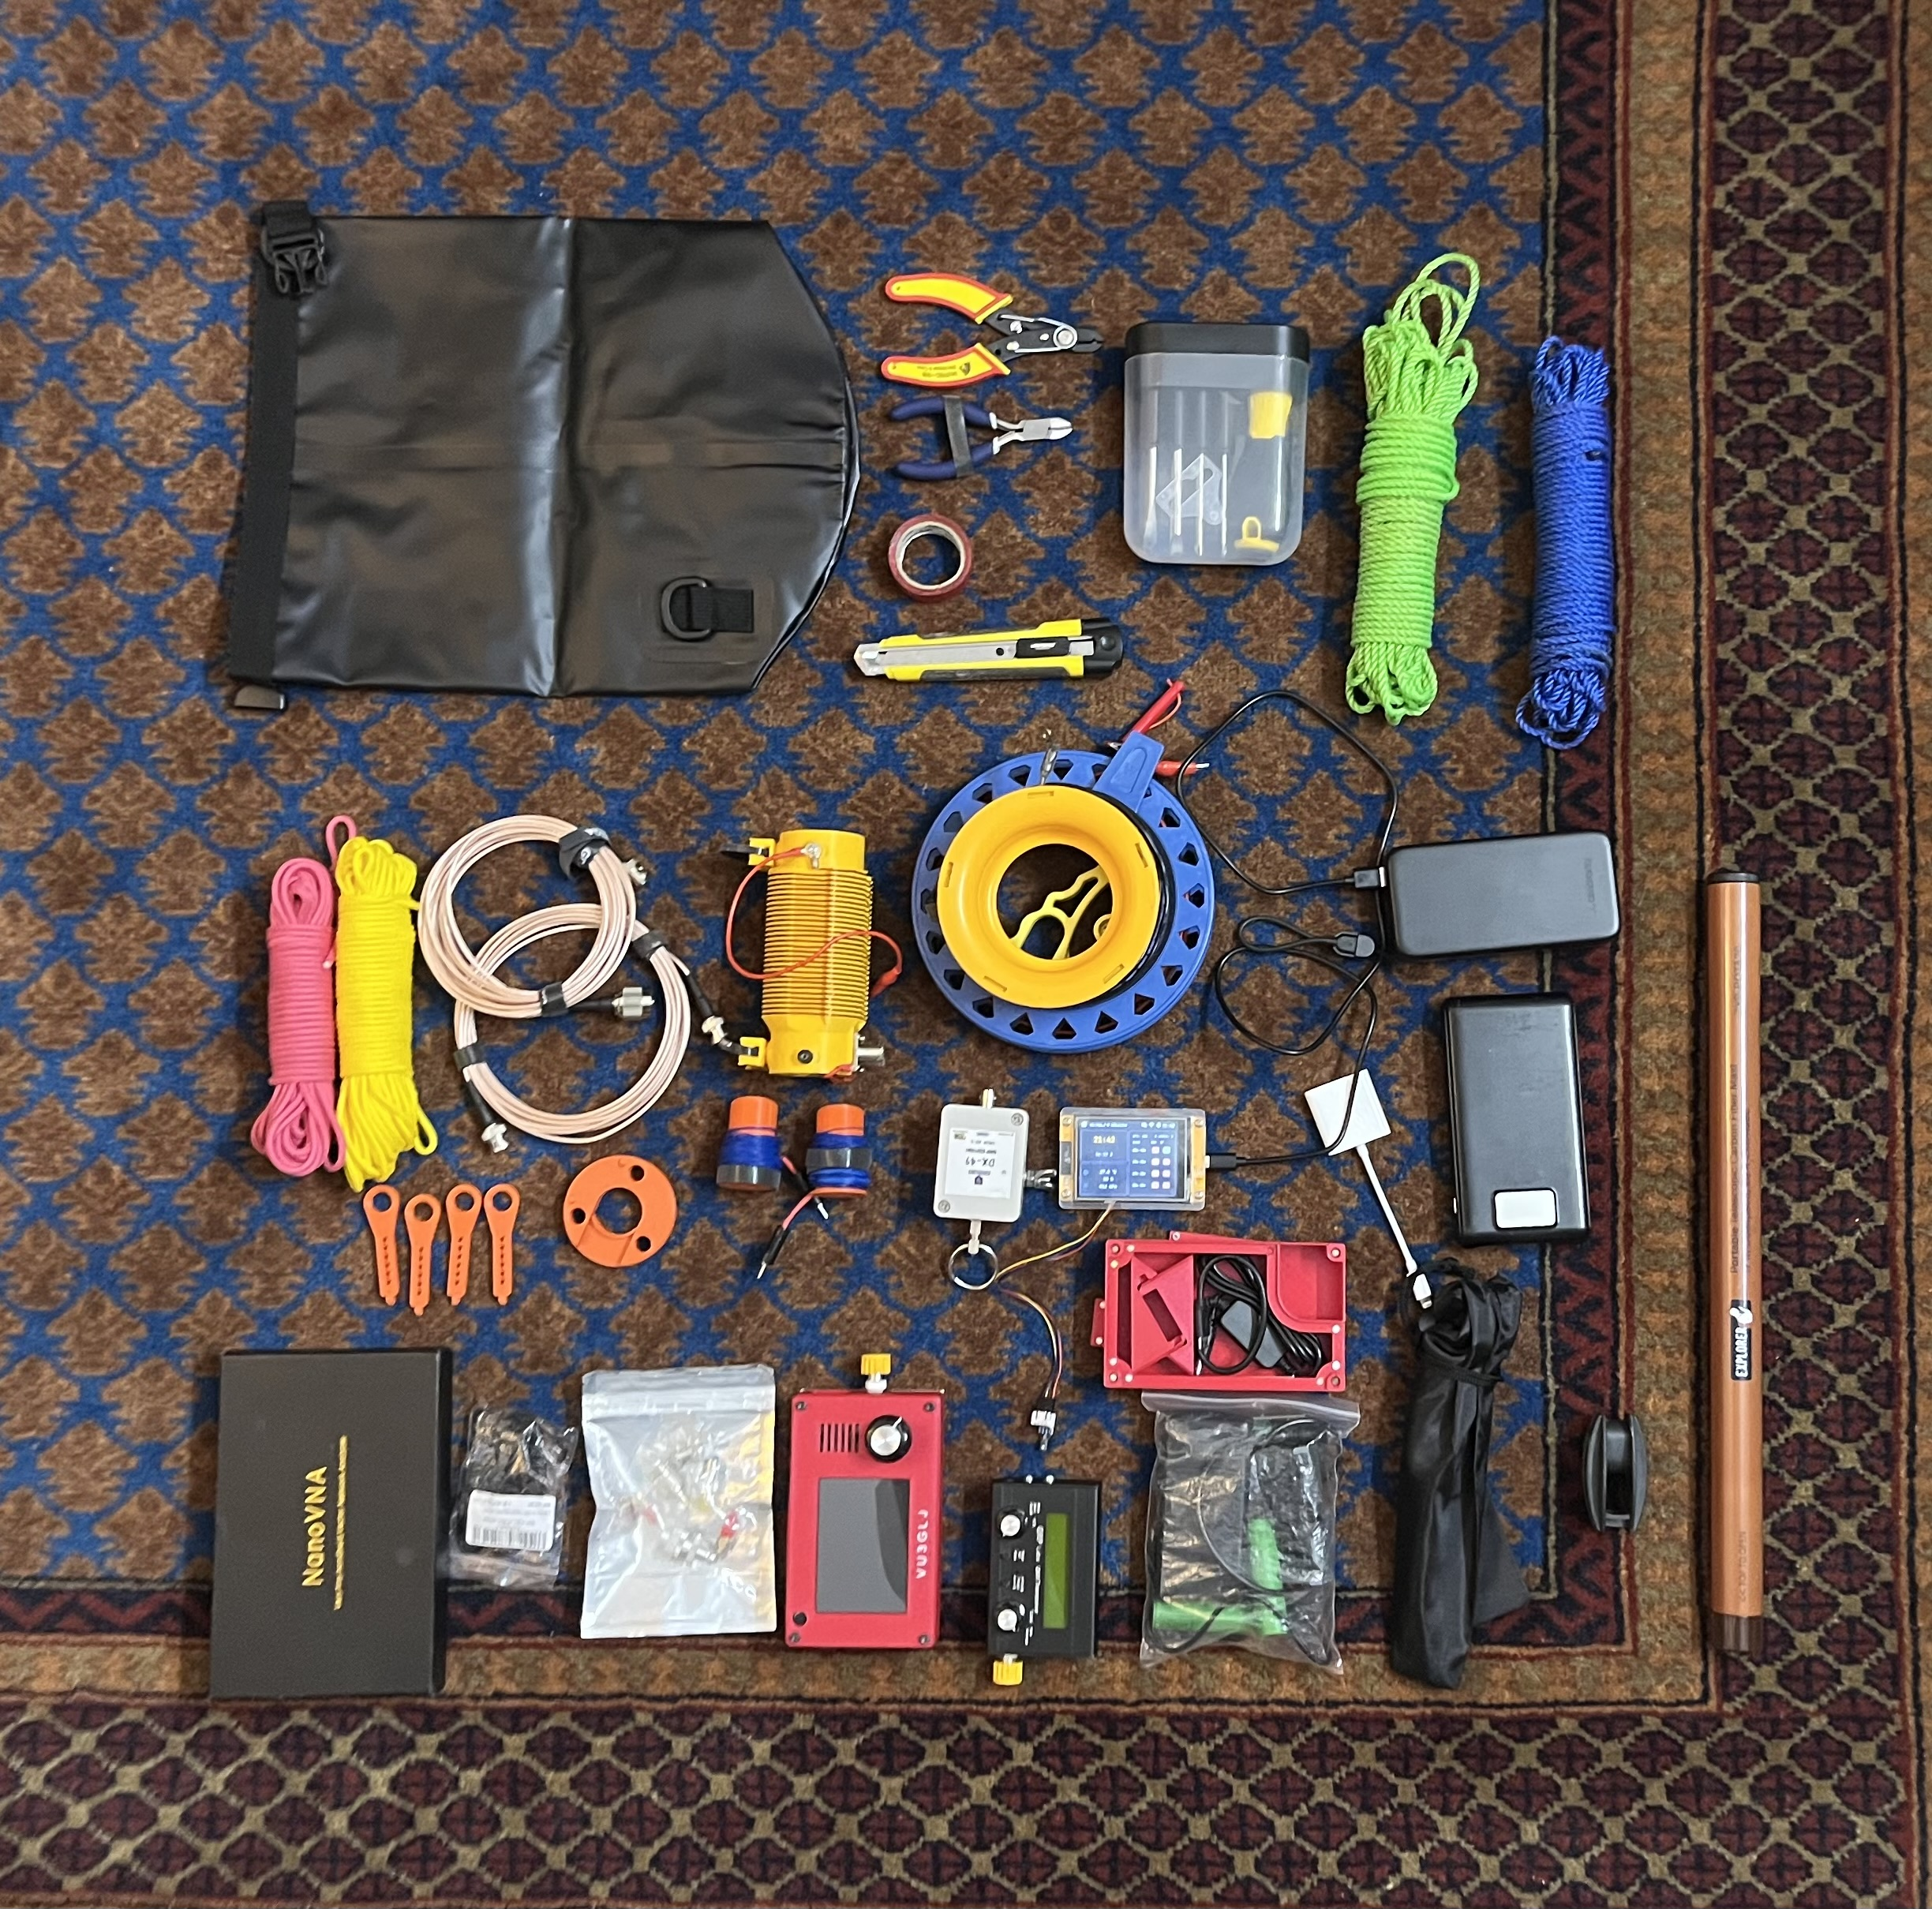
\includegraphics[width=0.5\linewidth]{qrp_backpack.jpeg}}
\caption{Author's QRP back-pack with two radios, two antennas and misc.
test equipment.}
\label{fig:qrp-backpack}
\end{figure}

\subsection{Preparing a station for POTA operations}
\label{subsection:station}
There are numerous approaches to activating parks:
\begin{itemize}
\item \textbf{Group or Solo}: Activations can be executed as a
  solo deployment or as a group trip, or even expanded into a
  collaborative community project that engages locals and youth. While
  solo operations necessitate a meticulously planned go-bag, group
  deployments can distribute the logistical load of transporting
  heavier antennas and power supplies\footnote{Please see
    \url{https://youtu.be/MZzqekrGJtI?si=36zFxp8Xths6k-sK} and
    \url{https://www.facebook.com/VU2UUU} (Last accessed: 15 Jul 2026)}.
\item \textbf{QRP or QRO}:  Operators must decide whether to deploy a
  lightweight, battery-powered QRP transceiver (the author's 1.5\,kg
  setup has two antennas, battery power and one
  radio\footnote{\url{https://ham.bharathpalavalli.com/posts/20260611182043-field_oeprations_and_preparing_a_go_bag/}}) or a higher-powered station requiring extensive
  wire antennas and high-capacity lithium batteries with greater
  reach/connectivity\footnote{Please check
    \url{https://www.youtube.com/@Harisriramaiah/videos} (Last accessed: 15
    Jul 2026) for detailed POTA activations with an elaborate station
    setup by VU2UCR}.
\item \textbf{Wilderness or Quick-mode}: Deployments can range from
  rigorous expeditions in remote, highly protected biospheres (where
  cellular networks may be non-existent) to vehicle operated. Remote
  wilderness activations demand meticulous pre-testing and weather
  preparation, whereas quick-mode operations benefit from minimal
  setup times and immediate network availability\footnote{Please see
    \url{https://youtu.be/-dt-KXlIckg?si=OttEdbJtdviN4Efy} for challenging
    conditions as well as engagement activities by VU3KOX (Last
    accessed: 15 Jul 2026)}.
\item \textbf{Activation or achieve targets}: Beyond merely securing
  the standard POTA activation, operators may focus on targeting
  specific international DX stations, bands or modes that they have as
  targets. Alternatively, treating POTA activations as yet another
  field environment serves as a platform for experimentation,
  allowing operators to test home-brewed equipment or evaluate
  real-time propagation using automated spotting
  networks.
\end{itemize}

\section{Discussion and Future Work}
The identification of 481 active, internationally visible HF operators
underscores both the challenges and the massive untapped potential for
amateur radio growth in the region. To catalyze domestic POTA
activity, future initiatives should focus on community-driven
``activation workshops'' and field mentoring at major conventions, such
as HAMFEST INDIA, to familiarize operators with portable setups.

Furthermore, collaborating with POTA administrators to map and include
more accessible, localized urban parks could drastically lower the
logistical barriers to entry. Advocacy for streamlined WPC and
respective Forest Dept. permissions for hassle-free temporary field
operations will also be critical. A qualitative study on the
challenges faced by the current activators will provide necessary
insights into increasing field operations and POTA activities. In
addition, it would be ideal to have the QTH locations of the operators
(active HF operators), to understand and analyze the spatial
properties such as distance to the park, terrain challenges, modes of
travel, available accommodation, etc. to evaluate practical deployment
possibilities.

\section{Acknowledgment and Disclaimer}
The author utilized Large Language Models (LLMs) to assist with data
aggregation scripts and \LaTeX\ typesetting, independently verifying
all generated code and analytical results. As a licensed operator, the
author thanks the Indian amateur radio community for reviewing a
preliminary version of this paper published on the author's blog~\cite{b17}.

The data and scripts are available at \repourl. {\raggedright Data aggregated within these scripts is
  sourced from POTA.app (\url{https://api.pota.app}), the Reverse
  Beacon Network (RBN) (\url{http://www.reversebeacon.net/}),
  PSKReporter (\url{https://retrieve.pskreporter.info/}), WSPRnet
  (\url{http://wsprnet.org/}), LoTW (\url{https://lotw.arrl.org/}),
  and public contest archives from CQ (e.g., \url{https://cqww.com/},
  \url{https://cqwpx.com}) and ARRL
  (\url{https://contests.arrl.org/}).\par}

% \IEEEtriggeratref{2}
\bibliographystyle{IEEEtran}
\bibliography{references}

\end{document}

%%% Local Variables:
%%% jinx-languages: "en_US"
%%% jinx-local-words: "APIs Bandipur ClubLog DXing GeoJSON HAMs HamQTH Karnataka LLMs Leaderboards LoTW Madhya Mudumalai PSKReporter Pradesh QSOs SWLs Uploaders WSPRnet WhatsApp activations boxplot choropleth de geo heatmap htbp htp jpeg lc lcc lccc lorenz png pota pre qrp unactivated"
%%% TeX-engine: default
%%% eval: (provide 'preview-latex)
%%% End:
